\chapter{Matériaux inorganiques et nanomatériaux}\label{ch:b3:inorganic-materials}

Une plaque d'\omterm{def:b3:inorganic-materials:sol-gel}{aérogel} de silice, un solide fait surtout d'air, tient une
fleur au-dessus d'une flamme de gaz sans la laisser se faner. C'est un
verre, obtenu non pas en fondant du sable mais en laissant un liquide se
figer en \omterm{def:b3:colloids:colloid}{gel}, puis en séchant ce \omterm{def:b3:colloids:colloid}{gel} sans le laisser s'effondrer. La chimie
des matériaux procède dans cet ordre~: choisir la structure, puis la voie
qui la produit, puis en déduire les propriétés. Ce chapitre suit les voies
d'accès aux solides inorganiques, les structures des \omterm{def:b3:inorganic-materials:ceramic}{céramiques}, des verres
et des cristaux poreux, et ce qui arrive à la matière quand une particule
ne mesure que quelques nanomètres.

\begin{recall}
Le volume de première année a décrit les types de structures cristallines,
les sites interstitiels, les variétés allotropiques, le graphite et le
diamant~; le volume de deuxième année, les diagrammes de phases, la
température de transition vitreuse et les polymères. Le
\cref{ch:b3:surfaces-catalysis} a défini la \omterm{def:b3:surfaces-catalysis:surface-area}{surface spécifique}, le
\cref{ch:b3:colloids} les \omterm{def:b3:colloids:colloid}{sols} et les \omterm{def:b3:colloids:colloid}{gels}, le \cref{ch:b3:solid-state} les
bandes, les \omterm{def:b3:solid-state:defects}{défauts ponctuels} et les \omterm{def:b3:solid-state:ionic-conductor}{conducteurs ioniques}~; le
\cref{ch:b3:quantum-model-systems} a résolu la \omterm{def:b3:quantum-model-systems:box}{particule dans une boîte}, et
le \cref{ch:b3:point-groups} a donné le groupe icosaédrique.
\end{recall}

\begin{omfigure}
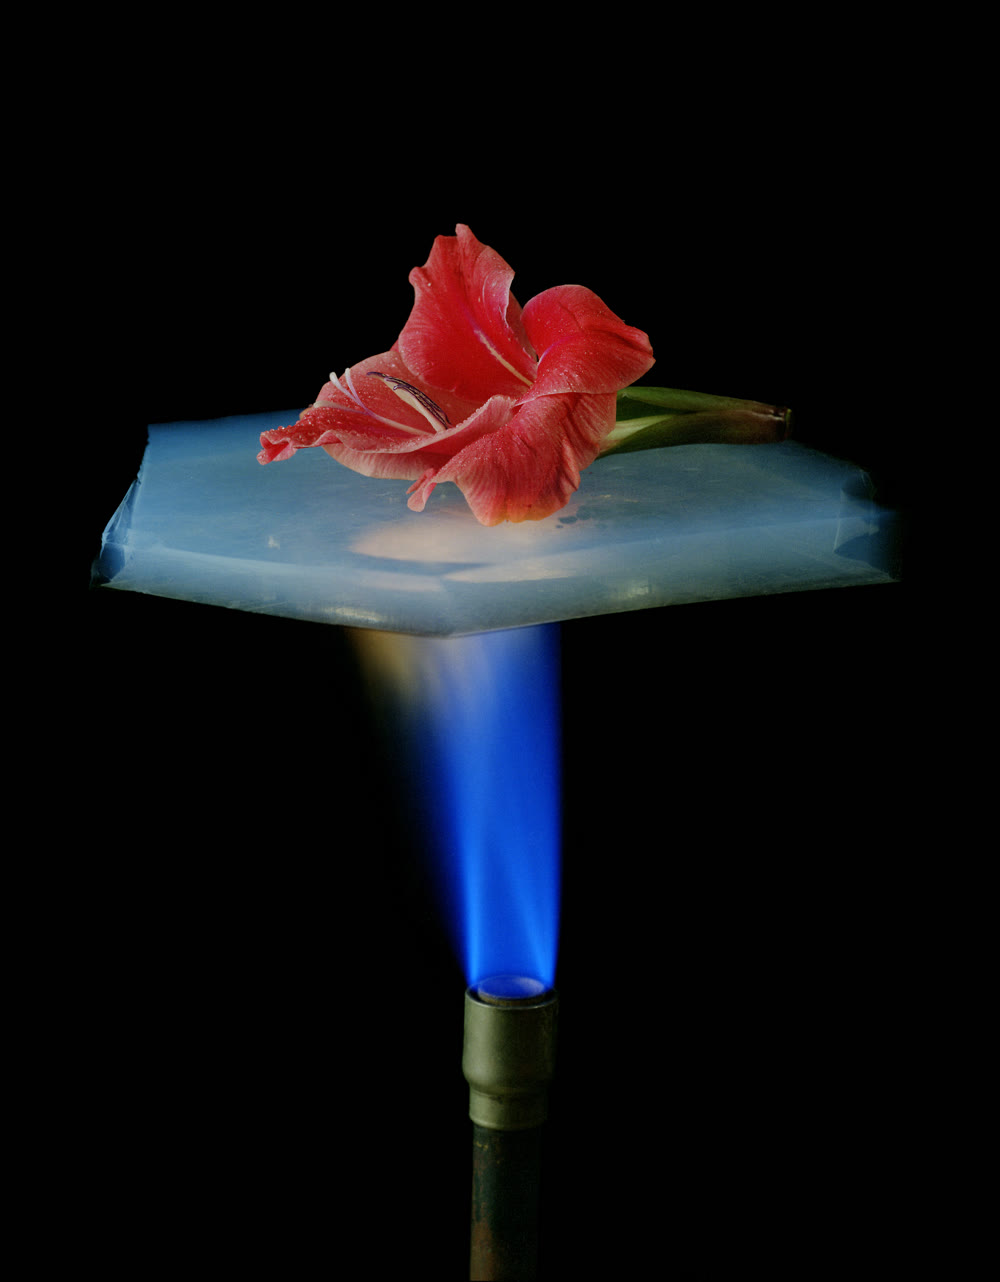
\includegraphics[width=0.38\linewidth]{images/book4/aerogel-flower.jpg}

{\small Une fleur sur une plaque d'\omterm{def:b3:inorganic-materials:sol-gel}{aérogel} de silice au-dessus d'une flamme
de gaz~: l'\omterm{def:b3:inorganic-materials:sol-gel}{aérogel}, un \omterm{def:b3:colloids:colloid}{gel} séché fait surtout de vide, conduit très mal la
chaleur. Photographie~: NASA/JPL, domaine public.}
\end{omfigure}

\section{Voies de synthèse}

\begin{definition}[Méthode céramique]\label{def:b3:inorganic-materials:ceramic-method}
La \emph{méthode céramique}\index{methode ceramique@méthode céramique} prépare un composé solide en
broyant ensemble les réactifs solides et en les chauffant, souvent pendant
des jours et avec des rebroyages, à des températures assez élevées pour que
les ions diffusent à travers les solides.
\end{definition}

La réaction de deux solides a lieu à leur contact, et le produit forme
entre eux une couche que les ions doivent ensuite traverser~: l'étape la
plus lente est la diffusion, qui ralentit à mesure que la couche
s'épaissit.

\begin{proposition}[Croissance parabolique]\label{prop:b3:inorganic-materials:parabolic}
Si la croissance d'une couche de produit est limitée par la diffusion à
travers elle, son épaisseur croît selon $x^2 = kt$.
\end{proposition}

\begin{proof}
Les concentrations étant fixées sur les deux faces de la couche, le flux qui
la traverse suit la loi de Fick, $J = D\Delta c/x$. La couche croît proportionnellement au flux~:
$\dd x/\dd t = \lambda J = \lambda D\Delta c/x$, avec $\lambda$ le volume de produit par mole transportée. Alors
$x\,\dd x = \lambda D\Delta c\,\dd t$, et l'intégration à partir de $x = 0$ en $t = 0$ donne $x^2 = 2\lambda D\Delta c\,t = kt$.
\end{proof}

Doubler la taille des particules multiplie donc le temps de réaction par
quatre~: d'où le broyage fin, le mélange à l'échelle atomique dans un
précurseur (un oxalate mixte ou un \omterm{def:b3:colloids:colloid}{gel} de citrate qui se décompose en la
phase visée), ou une voie en solution.

\begin{definition}[Procédé sol--gel]\label{def:b3:inorganic-materials:sol-gel}
Le \emph{procédé sol--gel}\index{procede sol--gel@procédé sol--gel} prépare un oxyde par
hydrolyse et condensation de précurseurs moléculaires, en général des
alcoxydes, en solution~: la solution devient un \omterm{def:b3:colloids:colloid}{sol} de petits agrégats
d'oxyde, puis un \omterm{def:b3:colloids:colloid}{gel}, réseau solide continu imprégné de liquide. Séché par
évaporation, le \omterm{def:b3:colloids:colloid}{gel} se contracte en un \emph{xérogel}\index{xerogel@xérogel} dense~; séché
au-dessus du point critique du liquide, ce qui l'élimine sans interface
liquide--gaz, il garde son volume sous forme d'\emph{aérogel}\index{aerogel@aérogel}.
\end{definition}

\begin{omfigure}
\setchemfig{atom sep=2.0em}
\schemestart
\chemfig{RO-Si(-[2]OR)(-[6]OR)-OR}
\+ \chemfig{H_2O}
\arrow{->[hydrolyse]}[,1.4]
\chemfig{RO-Si(-[2]OR)(-[6]OR)-OH}
\+ ROH
\schemestop
\par\bigskip
\schemestart
\chemfig{{\equiv}Si-OH}
\+
\chemfig{HO-Si{\equiv}}
\arrow{->[condensation]}[,1.6]
\chemfig{{\equiv}Si-O-Si{\equiv}}
\+ \chemfig{H_2O}
\schemestop
\par\medskip

{\small Chimie sol--gel d'un alcoxyde de silicium (R~: un groupe alkyle,
éthyle dans l'orthosilicate de tétraéthyle)~: l'eau remplace des groupes
alcoxy par des groupes hydroxy, et deux silanols se condensent en un pont
siloxane. Répétées, les condensations construisent un réseau de silice
tridimensionnel.}
\end{omfigure}

Les deux réactions donnent ensemble, pour une réaction complète,
$\ce{Si(OC2H5)4 + 2H2O -> SiO2 + 4C2H5OH}$. La catalyse acide rend l'hydrolyse rapide et la
condensation lente, ce qui donne des polymères fins, en chaînes~; la
catalyse basique produit l'inverse, des particules denses. Les revêtements
(couches antireflet sur le verre) sont obtenus en trempant une pièce dans
le \omterm{def:b3:colloids:colloid}{sol} puis en l'en retirant.

\begin{definition}[Synthèse hydrothermale]\label{def:b3:inorganic-materials:hydrothermal}
La \emph{synthèse hydrothermale}\index{synthese hydrothermale@synthèse hydrothermale} fait cristalliser un
solide à partir d'eau au-dessus de sa température d'ébullition normale, dans
un récipient fermé sous sa propre pression de vapeur~; la \emph{synthèse solvothermale}\index{synthese solvothermale@synthèse solvothermale}
fait de même dans un autre solvant.
\end{definition}

\begin{definition}[Dépôt chimique en phase vapeur]\label{def:b3:inorganic-materials:cvd}
Le \emph{dépôt chimique en phase vapeur}\index{depot chimique en phase vapeur@dépôt chimique en phase vapeur} (CVD) fait croître un
film solide sur une surface chauffée par la réaction de précurseurs gazeux
à son contact, comme le silicium à partir du silane, $\ce{SiH4 -> Si + 2H2}$, ou le diamant à partir de méthane et de dihydrogène.
\end{definition}

\begin{method}[Choisir une voie de synthèse]\label{met:b3:inorganic-materials:route}
\begin{enumerate}
  \item Un oxyde stable et réfractaire en poudre massive~: la \omterm{def:b3:inorganic-materials:ceramic-method}{méthode
        céramique}, avec un précurseur si le mélange est difficile.
  \item Une phase métastable, une poudre fine ou un revêtement à basse
        température~: sol--gel ou précipitation.
  \item De gros monocristaux d'une phase soluble seulement dans l'eau
        chaude (quartz) ou une charpente construite autour d'un gabarit
        (\omterm{def:b3:inorganic-materials:zeolite}{zéolithes})~: voie hydrothermale.
  \item Un film mince et pur sur un substrat (couches de \omterm{def:b3:solid-state:classes}{semi-conducteurs})~:
        CVD.
\end{enumerate}
\end{method}

\begin{inthelab}[Un revêtement sol--gel et un autoclave]
On agite l'orthosilicate de tétraéthyle avec de l'éthanol, de l'eau et une
goutte d'acide jusqu'à ce que la solution soit limpide~; une lame de verre
propre y est trempée puis retirée à vitesse lente et constante, séchée et
chauffée, ce qui laisse un film de silice assez mince pour montrer des
couleurs d'interférence. Pour une \omterm{def:b3:inorganic-materials:hydrothermal}{synthèse hydrothermale}, les réactifs sont
placés dans une chemise en polytétrafluoroéthylène, remplie au plus aux deux
tiers environ pour que le liquide en se dilatant ne remplisse pas le
récipient, scellée dans un autoclave en acier et chauffée dans une
étuve~; l'autoclave n'est ouvert qu'une fois froid.
\end{inthelab}

\begin{omfigure}
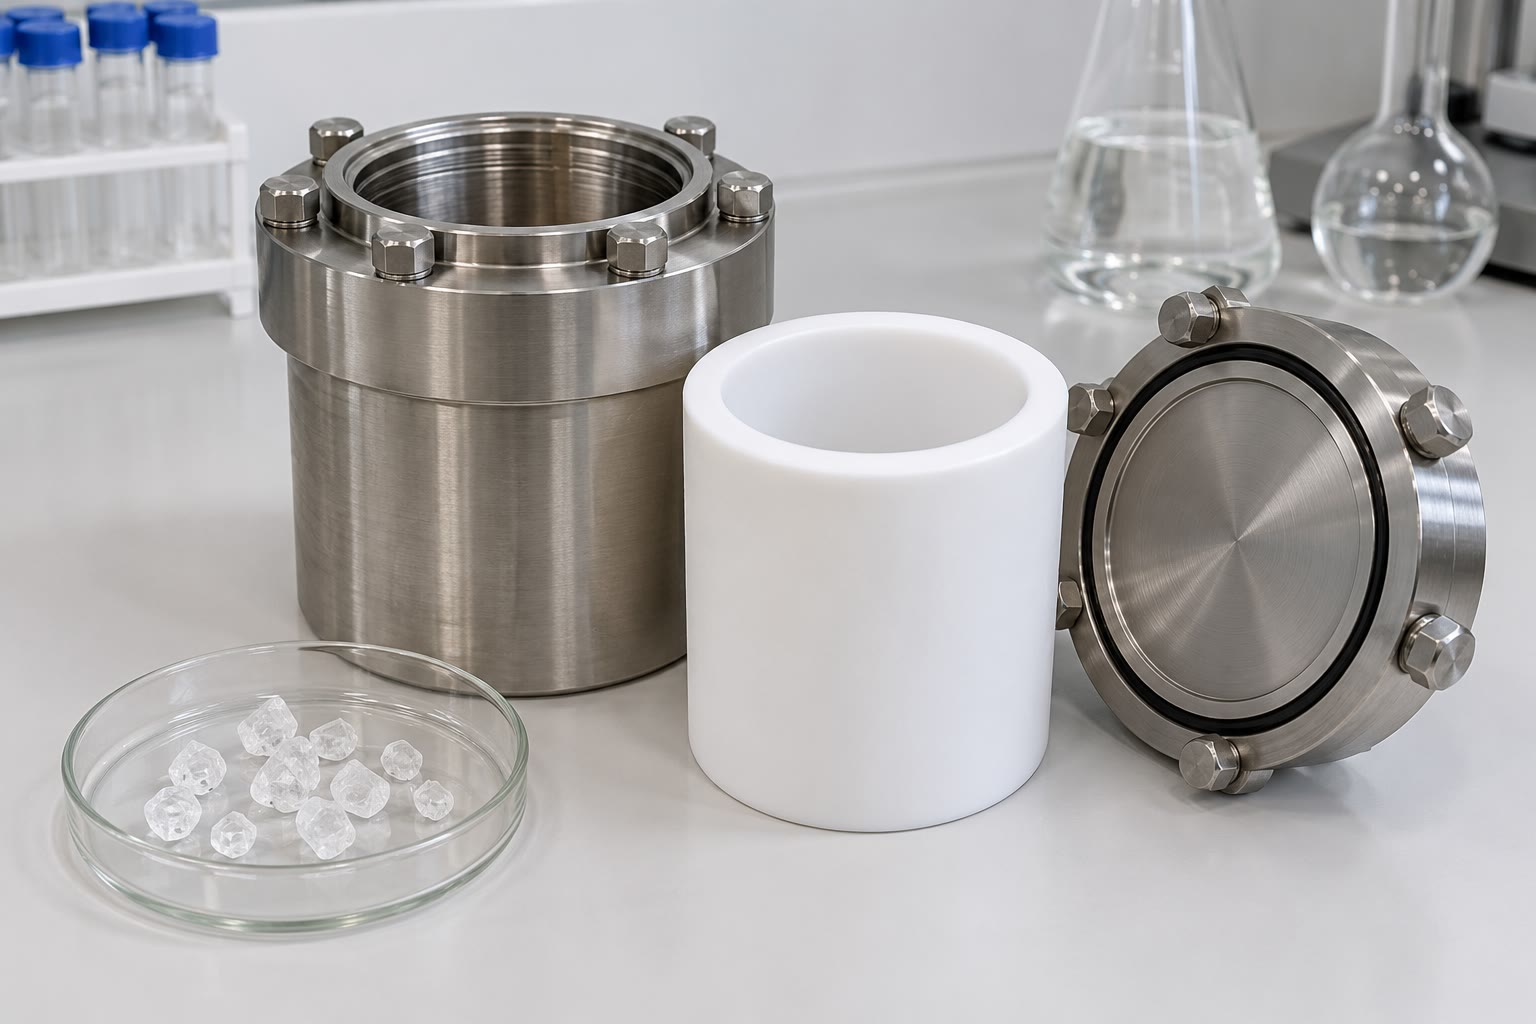
\includegraphics[width=0.5\linewidth]{images/book4/ai/b3-23-autoclave.jpg}

{\small Un autoclave de laboratoire pour la \omterm{def:b3:inorganic-materials:hydrothermal}{synthèse hydrothermale}~: un corps
en acier à couvercle boulonné, une chemise en polymère blanc qui contient le
mélange réactionnel, et des cristaux qui y ont crû.}
\end{omfigure}

\section{Céramiques et verres}

\begin{definition}[Céramique]\label{def:b3:inorganic-materials:ceramic}
Une \emph{céramique}\index{ceramique@céramique} est un solide inorganique non métallique
obtenu en chauffant une poudre~: oxydes, nitrures et carbures, ou produits
argileux.
\end{definition}

\begin{definition}[Structure pérovskite]\label{def:b3:inorganic-materials:perovskite}
La \emph{structure pérovskite}\index{structure perovskite@structure pérovskite} d'un oxyde $\mathrm{ABO_3}$
place les petits cations B aux centres d'octaèdres $\mathrm{BO_6}$ liés par leurs sommets et
les gros cations A dans les cavités de coordinence douze qui les séparent~;
dans la maille cubique idéale, B est au centre, O aux centres des faces, A
aux sommets. Le \emph{facteur de tolérance}\index{facteur de tolerance@facteur de tolérance} mesure à quel point
les ions s'ajustent~:
\[
  t = \frac{r_A + r_O}{\sqrt2\,(r_B + r_O)}.
\]
\end{definition}

\begin{omfigure}
\tdplotsetmaincoords{60}{100}
\begin{tikzpicture}[tdplot_main_coords, scale=1.5, font=\small,
  aA/.style={om atom, ball color=green!45!black, minimum size=7.4mm},
  aB/.style={om atom, ball color=black!35, minimum size=4.4mm},
  aOs/.style={om atom, ball color=red!80, minimum size=4.8mm}]
  \pic[transform shape] {omcubeo={2}};
  % atoms back to front for view 60/100 (depth 0.853x + 0.150y + 0.5z)
  \node[aA] at (0,0,0) {};
  \node[aA] at (0,2,0) {};
  \node[aOs] (o1) at (0,1,1) {};
  \node[aA] at (0,0,2) {};
  \node[aOs] (o2) at (1,1,0) {};
  \node[aA] at (0,2,2) {};
  \node[aOs] (o3) at (1,0,1) {};
  \node[aB] (b) at (1,1,1) {};
  \node[aOs] (o4) at (1,2,1) {};
  \node[aA] at (2,0,0) {};
  \node[aOs] (o5) at (1,1,2) {};
  \node[aA] at (2,2,0) {};
  \node[aOs] (o6) at (2,1,1) {};
  \node[aA] at (2,0,2) {};
  \node[aA] at (2,2,2) {};
  \begin{scope}[on background layer]
    \draw[omMeth!70, line width=0.6pt] (o1.center) -- (o2.center) -- (o6.center) -- (o5.center) -- cycle
      (o3.center) -- (o2.center) -- (o4.center) -- (o5.center) -- cycle
      (o1.center) -- (o3.center) -- (o6.center) -- (o4.center) -- cycle;
    \draw[bond] (b.center) -- (o1.center) (b.center) -- (o2.center) (b.center) -- (o3.center)
      (b.center) -- (o4.center) (b.center) -- (o5.center) (b.center) -- (o6.center);
  \end{scope}
  \node[anchor=west] at (2,3.35,2) {A};
  \node[anchor=west] at (2,3.35,1) {O};
  \node[anchor=west] at (2,3.35,0) {B};
  \node[aA, minimum size=4mm] at (2,3.2,2) {};
  \node[aOs, minimum size=3.2mm] at (2,3.2,1) {};
  \node[aB, minimum size=3mm] at (2,3.2,0) {};
\end{tikzpicture}

{\small La maille cubique de la pérovskite $\mathrm{ABO_3}$~: un cation B (en gris) au centre d'un
octaèdre de six ions oxyde situés aux centres des faces (arêtes vertes), les
cations A aux sommets. Chaque ion A d'un sommet est partagé entre huit
mailles et chaque oxygène entre deux~: un A, un B et trois O par maille.}
\end{omfigure}

\begin{proposition}[Facteur de tolérance idéal]\label{prop:b3:inorganic-materials:tolerance}
Dans la pérovskite cubique idéale, les ions étant en contact selon les
directions B--O et A--O, $t = 1$.
\end{proposition}

\begin{proof}
Pour une arête $a$, B au centre et O au centre d'une face sont distants de $a/2$~: $r_B + r_O = a/2$.
A à un sommet et O au centre d'une face adjacente sont distants d'une
demi-diagonale de face~: $r_A + r_O = a\sqrt2/2$. En divisant, $(r_A + r_O)/(r_B + r_O) = \sqrt2$, donc $t = 1$.
\end{proof}

Lorsque $t$ est légèrement inférieur à 1, l'ion A est trop petit pour sa cavité et les
octaèdres basculent pour se refermer autour de lui, ce qui abaisse la symétrie~; lorsque $t$ est supérieur à 1,
l'ion B est trop petit pour son octaèdre et peut se décentrer.

\begin{definition}[Ferroélectrique]\label{def:b3:inorganic-materials:ferroelectric}
Un \emph{ferroélectrique}\index{ferroelectrique@ferroélectrique} est un cristal doté d'une
polarisation électrique spontanée qu'un champ électrique appliqué peut
inverser.
\end{definition}

% ledger: rion:Ba2+XII, rion:Ti4+VI, rion:O2-VI
Le titanate de baryum est le cas classique~: avec $r(\ce{Ba^2+}) = \qty{161}{pm}$ (coordinence douze),
$r(\ce{Ti^4+}) = \qty{60.5}{pm}$ et $r(\ce{O^2-}) = \qty{140}{pm}$, $t = 1.06$. Au-dessous d'une température de transition, les
ions titane se décentrent, tous dans la même direction au sein d'un
domaine, et le cristal se polarise~; l'énorme permittivité au voisinage de
la transition fait du titanate de baryum le diélectrique de la plupart des
condensateurs \omterm{def:b3:inorganic-materials:ceramic}{céramiques}.

\begin{definition}[Verres d'oxydes]\label{def:b3:inorganic-materials:glass}
Un \emph{verre d'oxydes}\index{verre d'oxydes} est un solide oxyde amorphe,
obtenu en refroidissant un liquide fondu sans cristallisation. Ses
\emph{formateurs de réseau}\index{formateur de reseau@formateur de réseau} ($\ce{SiO2}$, $\ce{B2O3}$, $\ce{P2O5}$) construisent un réseau continu
de polyèdres liés par leurs sommets~; ses \emph{modificateurs de réseau}\index{modificateur de reseau@modificateur de réseau}
($\ce{Na2O}$, $\ce{CaO}$) rompent des ponts de ce réseau, chaque ion oxyde ajouté
transformant un oxygène pontant en deux oxygènes non pontants, les cations
se logeant dans les trous.
\end{definition}

\begin{omfigure}
\begin{tikzpicture}
\begin{axis}[name=c, width=0.5\linewidth, axis equal image, hide axis, xmin=-1.2, xmax=12.6, ymin=-1.2, ymax=8.7]
\addplot[quiver={u=\thisrow{u}, v=\thisrow{v}}, -, black!60, line width=0.6pt] table {figdata/out/bachelor-3-glass-network-crystal-bonds.dat};
\addplot[only marks, mark=*, mark size=2.2pt, omDef] table {figdata/out/bachelor-3-glass-network-crystal-T.dat};
\addplot[only marks, mark=*, mark size=1.3pt, omThm, mark options={fill=white}] table {figdata/out/bachelor-3-glass-network-crystal-O.dat};
\end{axis}
\begin{axis}[at={(c.east)}, anchor=west, xshift=0.2cm, width=0.5\linewidth, axis equal image, hide axis, xmin=-1.2, xmax=12.6, ymin=-1.2, ymax=8.7]
\addplot[quiver={u=\thisrow{u}, v=\thisrow{v}}, -, black!60, line width=0.6pt] table {figdata/out/bachelor-3-glass-network-glass-bonds.dat};
\addplot[only marks, mark=*, mark size=2.2pt, omDef] table {figdata/out/bachelor-3-glass-network-glass-T.dat};
\addplot[only marks, mark=*, mark size=1.3pt, omThm, mark options={fill=white}] table {figdata/out/bachelor-3-glass-network-glass-O.dat};
\addplot[only marks, mark=*, mark size=1.5pt, omThm] table {figdata/out/bachelor-3-glass-network-glass-NBO.dat};
\addplot[only marks, mark=*, mark size=2.6pt, omProp] table {figdata/out/bachelor-3-glass-network-glass-Na.dat};
\end{axis}
\end{tikzpicture}

{\small Représentation bidimensionnelle d'un cristal et d'un verre de même
composition (en bleu~: formateurs tricoordinés~; cercles rouges vides~:
oxygènes pontants). À gauche, le cristal répète un même cycle. À droite, le
verre~: chaque formateur a toujours trois oxygènes à des distances presque
égales, mais les cycles comptent cinq, six ou sept chaînons et rien ne se
répète~; en deux endroits, un modificateur a rompu un pont, laissant deux
oxygènes non pontants (rouges pleins) et un cation (orange) dans la cavité.
Réseau modèle, relaxé avec des ressorts.}
\end{omfigure}

William Zachariasen soutint en 1932 qu'un oxyde forme facilement un verre
lorsque son cation est entouré de peu d'oxygènes (trois ou quatre), que
chaque oxygène relie au plus deux cations et que les polyèdres partagent
des sommets, non des arêtes ou des faces~: un réseau désordonné ne coûte
alors guère plus d'énergie que le cristal. Le verre à vitre est de la
silice additionnée d'oxydes de sodium et de calcium comme modificateurs, qui
abaissent la température de fusion. Le verre trempé chimiquement des
téléphones est plongé dans du nitrate de potassium fondu~: des ions $\ce{K+}$, plus gros,
remplacent les ions $\ce{Na+}$ de la surface et, à l'étroit, la mettent en compression, si
bien que les fissures ne s'ouvrent pas.

\section{Solides poreux~: zéolithes et réseaux}

\begin{definition}[Zéolithes]\label{def:b3:inorganic-materials:zeolite}
Une \emph{zéolithe}\index{zeolithe@zéolithe} est un aluminosilicate cristallin dont la
charpente de tétraèdres $\ce{SiO4}$ et $\ce{AlO4}$ liés par leurs sommets renferme des cages et des
canaux de taille moléculaire, contenant des cations échangeables et de
l'eau. Un \emph{tamis moléculaire}\index{tamis moleculaire@tamis moléculaire} est un solide poreux qui
admet les molécules selon leur taille~; la \emph{sélectivité de forme}\index{selectivite de forme@sélectivité de forme}
est le contrôle d'une réaction par la taille et la forme des pores dans
lesquels elle a lieu.
\end{definition}

Chaque tétraèdre $\ce{AlO4}$ porte une charge négative de plus qu'un tétraèdre $\ce{SiO4}$
(aluminium(III) à la place de silicium(IV))~; les cations des cages, $\ce{Na+}$ ou $\ce{Ca^2+}$,
la compensent et peuvent être échangés.

\begin{proposition}[Règle de Löwenstein]\label{prop:b3:inorganic-materials:lowenstein}
Dans une charpente de \omterm{def:b3:inorganic-materials:zeolite}{zéolithe}, deux tétraèdres $\ce{AlO4}$ ne partagent jamais un oxygène~: les liaisons Al--O--Al
sont absentes (une observation sur toutes les charpentes d'aluminosilicates
connues). En conséquence, le rapport Si/Al d'une \omterm{def:b3:inorganic-materials:zeolite}{zéolithe} vaut au moins 1.
\end{proposition}

\begin{proof}[Démonstration de la conséquence]
Chaque aluminium a quatre oxygènes, chacun partagé avec un silicium d'après la règle~:
$4N_{\mathrm{Al}}$ liaisons Al--O--Si. Chaque silicium n'a que quatre oxygènes et participe donc à
au plus quatre de ces liaisons~: $4N_{\mathrm{Al}} \le 4N_{\mathrm{Si}}$, c'est-à-dire $N_{\mathrm{Si}}/N_{\mathrm{Al}} \ge 1$. L'égalité impose que chaque
silicium ait quatre voisins aluminium~: Si et Al alternent.
\end{proof}

\begin{omfigure}
\tdplotsetmaincoords{55}{135}
\begin{tikzpicture}[tdplot_main_coords, scale=0.85, font=\small, baseline=(current bounding box.center),
  tSi/.style={circle, inner sep=0pt, minimum size=2.6mm, draw=black!70, fill=omDef!80},
  tAl/.style={circle, inner sep=0pt, minimum size=2.6mm, draw=black!70, fill=omProp!80}]
  % edges of a truncated octahedron (vertices: permutations of (0, +-1, +-2));
  % hidden edges (both faces facing away for this view) dashed
  \foreach \a/\b/\c/\d/\e/\f in {-2/-1/0/-2/0/-1, -2/-1/0/-2/0/1, -2/-1/0/-1/-2/0, -2/0/-1/-2/1/0, -2/0/-1/-1/0/-2, -1/-2/0/0/-2/-1, -1/-2/0/0/-2/1, -1/0/-2/0/-1/-2, -1/0/-2/0/1/-2, 0/-2/-1/0/-1/-2, 0/-2/-1/1/-2/0, 0/-1/-2/1/0/-2}
    \draw[black!40, dashed] (\a,\b,\c) -- (\d,\e,\f);
  \foreach \a/\b/\c/\d/\e/\f in {-2/0/1/-2/1/0, -2/0/1/-1/0/2, -2/1/0/-1/2/0, -1/0/2/0/-1/2, -1/0/2/0/1/2, -1/2/0/0/2/-1, -1/2/0/0/2/1, 0/-2/1/0/-1/2, 0/-2/1/1/-2/0, 0/-1/2/1/0/2, 0/1/-2/0/2/-1, 0/1/-2/1/0/-2, 0/1/2/0/2/1, 0/1/2/1/0/2, 0/2/-1/1/2/0, 0/2/1/1/2/0, 1/-2/0/2/-1/0, 1/0/-2/2/0/-1, 1/0/2/2/0/1, 1/2/0/2/1/0, 2/-1/0/2/0/-1, 2/-1/0/2/0/1, 2/0/-1/2/1/0, 2/0/1/2/1/0}
    \draw[black!75, line width=0.7pt] (\a,\b,\c) -- (\d,\e,\f);
  % T atoms back to front; hidden ones paler
  \foreach \x/\y/\z/\k/\v in {-2/-1/0/Si/0, -1/-2/0/Al/0, -2/0/-1/Al/0, 0/-2/-1/Si/0, -1/0/-2/Si/0, 0/-1/-2/Al/0, -2/0/1/Al/1, 0/-2/1/Si/1, -2/1/0/Si/1, 1/-2/0/Al/1, 0/1/-2/Al/1, 1/0/-2/Si/1, -1/0/2/Si/1, 0/-1/2/Al/1, -1/2/0/Al/1, 2/-1/0/Si/1, 0/2/-1/Si/1, 2/0/-1/Al/1, 0/1/2/Al/1, 1/0/2/Si/1, 0/2/1/Si/1, 2/0/1/Al/1, 1/2/0/Al/1, 2/1/0/Si/1}
    \node[t\k, opacity=0.35+0.65*\v] at (\x,\y,\z) {};
\end{tikzpicture}
\hspace{1.2cm}
\begin{tikzpicture}[font=\small, scale=0.8, baseline=(current bounding box.center)]
  \foreach \i in {0,1,2} \foreach \j in {0,1,2} {
    \fill[omDef!70] ($(2.2*\i,2.2*\j)+(-0.28,-0.28)$) rectangle +(0.56,0.56);
  }
  \foreach \i in {0,1} \foreach \j in {0,1,2} {
    \draw[black!70, line width=0.8pt] (2.2*\i+0.28,2.2*\j) -- (2.2*\i+0.75,2.2*\j);
    \draw[black!70, line width=0.8pt] (2.2*\i+1.45,2.2*\j) -- (2.2*\i+1.92,2.2*\j);
    \node[draw=black!70, regular polygon, regular polygon sides=6, minimum size=5.6mm, inner sep=0pt] at (2.2*\i+1.1,2.2*\j) {};
  }
  \foreach \i in {0,1,2} \foreach \j in {0,1} {
    \draw[black!70, line width=0.8pt] (2.2*\i,2.2*\j+0.28) -- (2.2*\i,2.2*\j+0.75);
    \draw[black!70, line width=0.8pt] (2.2*\i,2.2*\j+1.45) -- (2.2*\i,2.2*\j+1.92);
    \node[draw=black!70, regular polygon, regular polygon sides=6, minimum size=5.6mm, inner sep=0pt] at (2.2*\i,2.2*\j+1.1) {};
  }
  \node[font=\scriptsize, align=center] at (1.1,-0.85) {nœud $\ce{Zn4O}$ $+$ ligand téréphtalate};
\end{tikzpicture}

{\small À gauche~: une cage sodalite, l'unité de construction de la
\omterm{def:b3:inorganic-materials:zeolite}{zéolithe} A, avec un atome tétraédrique à chaque sommet (les oxygènes, au
milieu de chaque arête, ne sont pas dessinés)~; le silicium (en bleu) et
l'aluminium (en orange) alternent, comme l'exige la règle de Löwenstein
quand Si/Al = 1. À droite~: une couche d'un \omterm{def:b3:inorganic-materials:mof}{réseau métallo-organique},
schématique~: des agrégats $\ce{Zn4O}$ (carrés) reliés par des ligands
benzène-1,4-dicarboxylate (cycles) en une grille cubique à larges pores.}
\end{omfigure}

\begin{method}[Formule et capacité d'échange d'une zéolithe]\label{met:b3:inorganic-materials:zeolite-formula}
\begin{enumerate}
  \item Écrire la charpente sous la forme $\mathrm{[(AlO_2)_x(SiO_2)_y]^{x-}}$~: Si/Al $= y/x$.
  \item La charge $-x$ de la charpente est compensée par des cations~: $x$ monovalents ou $x/2$
        divalents.
  \item La capacité d'échange est la quantité de charge échangeable par
        gramme~:
        $x/M$ moles de cations monovalents, $x/2M$ de cations divalents, avec $M$ la
        masse molaire de la formule telle qu'elle est pesée (anhydre ou
        hydratée).
\end{enumerate}
\end{method}

\begin{proposition}[Capacité d'échange]\label{prop:b3:inorganic-materials:exchange-capacity}
La capacité d'une \omterm{def:b3:inorganic-materials:zeolite}{zéolithe} pour un cation de charge $z$ vaut $x/(zM)$ moles par gramme,
où $x$ est le nombre d'atomes d'aluminium dans une formule de masse molaire $M$.
\end{proposition}

\begin{proof}
Chaque aluminium apporte une charge négative à la charpente~; la neutralité
électrique exige $x$ unités de charge positive, toutes échangeables, soit
$x/z$ cations de charge $z$ par unité formulaire, c'est-à-dire par masse $M$.
\end{proof}

% ledger: iza:LTA.window, iza:MFI.channels
La \omterm{def:b3:inorganic-materials:zeolite}{zéolithe} A a des fenêtres de huit tétraèdres, de \qty{0.41}{nm} de
diamètre~: l'eau et les petits ions passent, les molécules ramifiées non.
La ZSM-5 possède deux systèmes de canaux de dix tétraèdres, d'environ 0.51 à
\qty{0.56}{nm}~: lors de la conversion du méthanol ou de l'alkylation du
toluène, le \textit{para}-xylène, élancé, diffuse vers l'extérieur bien
plus vite que ses isomères \textit{ortho} et \textit{meta}, qui restent et
s'isomérisent. C'est la \omterm{def:b3:inorganic-materials:zeolite}{sélectivité de forme}.

\begin{definition}[Réseaux métallo-organiques]\label{def:b3:inorganic-materials:mof}
Un \emph{réseau métallo-organique}\index{reseau metallo-organique@réseau métallo-organique} (MOF) est un
solide cristallin construit à partir d'ions ou d'agrégats métalliques
reliés par des ligands organiques polytopiques en un réseau poreux. Une
\emph{unité de construction secondaire}\index{unite de construction secondaire@unité de construction secondaire} est l'agrégat métallique avec
ses groupes coordinants, traité comme un nœud du réseau~; la \emph{synthèse réticulaire}\index{synthese reticulaire@synthèse réticulaire}
est la conception d'un réseau par le choix de nœuds et de ligands de
géométrie donnée, de sorte qu'ils s'assemblent selon une topologie choisie.
\end{definition}

% ledger: cod:MOF5.formula, cod:MOF5.a
Dans le MOF-5, des agrégats $\ce{Zn4O}$ portant six groupes carboxylate forment des nœuds
octaédriques, et des ligands benzène-1,4-dicarboxylate les relient le long
des arêtes d'un réseau cubique, $a = \qty{25.82}{\angstrom}$ pour une maille de huit nœuds. Remplacer le
ligand par un ligand plus long conserve la topologie et agrandit les
pores~: c'est l'idée réticulaire. De tels réseaux ont des \omterm{def:b3:surfaces-catalysis:surface-area}{surfaces
spécifiques} de plusieurs milliers de mètres carrés par gramme et sont
étudiés pour stocker le dihydrogène et le méthane et pour capter le dioxyde
de carbone.

\begin{definition}[Tailles de pores]\label{def:b3:inorganic-materials:pores}
% ledger: pore:micro, pore:macro
Par convention, les \emph{micropores}\index{micropore} ont moins de \qty{2}{nm},
les \emph{mésopores}\index{mesopore@mésopore} entre 2 et \qty{50}{nm}, et
les \emph{macropores}\index{macropore} plus de \qty{50}{nm}.
\end{definition}

Les \omterm{def:b3:inorganic-materials:zeolite}{zéolithes} et la plupart des MOF sont microporeux~; les \omterm{def:b3:colloids:colloid}{gels} de silice et les \omterm{def:b3:inorganic-materials:sol-gel}{aérogels}, mésoporeux.

\section{Nanoparticules}

\begin{definition}[Nanomatériaux]\label{def:b3:inorganic-materials:nano}
Un \emph{nanomatériau}\index{nanomateriau@nanomatériau} a au moins une dimension comprise entre
environ 1 et \qty{100}{nm}~; une \emph{nanoparticule}\index{nanoparticule} les a
toutes les trois.
\end{definition}

\begin{proposition}[Agrégats magiques]\label{prop:b3:inorganic-materials:magic}
Un agrégat cuboctaédrique formé d'un atome central et de $n$ couches
complètes compte
\[
  N(n) = \frac{10n^3 + 15n^2 + 11n + 3}{3}
\]
atomes, dont $10n^2 + 2$ en surface~: 13, 55, 147, 309, \dots
\end{proposition}

\begin{proof}
La $k$-ième couche d'un cuboctaèdre a 12 sommets, 24 arêtes portant chacune $k - 1$ atomes
intérieurs, 8 faces triangulaires portant chacune $(k - 1)(k - 2)/2$ atomes intérieurs et 6
faces carrées portant chacune $(k - 1)^2$~: au total $12 + 24(k - 1) + 4(k - 1)(k - 2) + 6(k - 1)^2 = 10k^2 + 2$. Alors
$N(n) = 1 + \sum_{k=1}^{n}(10k^2 + 2) = 1 + \frac{10n(n + 1)(2n + 1)}{6} + 2n$, qui se développe en la formule~; la
couche externe, de $10n^2 + 2$ atomes, est la surface.
\end{proof}

\begin{omfigure}
\begin{tikzpicture}
\begin{axis}[name=a, width=0.47\linewidth, height=5.4cm, xmin=0, xmax=18, ymin=0, ymax=1,
  axis lines=left, xlabel={diamètre / \unit{nm}}, ylabel={fraction des atomes en surface},
  tick label style={font=\scriptsize}, label style={font=\small}]
\addplot[omDef, thick, mark=*, mark size=1pt] table[x=diam_nm, y=fsurf] {figdata/out/bachelor-3-nanoparticle-size.dat};
\end{axis}
\begin{axis}[at={(a.east)}, anchor=west, xshift=1.5cm, width=0.47\linewidth, height=5.4cm,
  xmin=0.8, xmax=6, ymin=0, ymax=3, axis lines=left,
  xlabel={rayon $R$ / \unit{nm}}, ylabel={énergie de confinement / \unit{eV}},
  tick label style={font=\scriptsize}, label style={font=\small}]
\addplot[omThm, thick] table[x=R_nm, y=dE_eV] {figdata/out/bachelor-3-nanoparticle-size-b.dat};
\end{axis}
\end{tikzpicture}

{\small À gauche~: fraction des atomes situés à la surface d'agrégats d'or
cuboctaédriques en fonction de leur diamètre~: plus de la moitié pour les
agrégats de moins de \qty{3}{nm} environ, encore un cinquième à
\qty{8}{nm}. À droite~: énergie de confinement d'une paire électron--trou
dans une \omterm{def:b3:inorganic-materials:quantum-dot}{boîte quantique} sphérique (\omterm{def:b3:quantum-model-systems:oscillator}{masse réduite} du modèle $0.10\,m_e$),
qui s'ajoute à la \omterm{def:b3:solid-state:band}{bande interdite} et décroît comme $1/R^2$.}
\end{omfigure}

Avec une grande fraction de ses atomes en surface, où ils ont moins de
voisins, une \omterm{def:b3:inorganic-materials:nano}{nanoparticule} fond à plus basse température que le métal
massif, est plus réactive et peut être un bien meilleur catalyseur~: l'or
massif est inerte, alors que des particules d'or de quelques nanomètres
oxydent le monoxyde de carbone à température ambiante.

\begin{definition}[Boîtes quantiques]\label{def:b3:inorganic-materials:quantum-dot}
Une \emph{boîte quantique}\index{boite quantique@boîte quantique} est un nanocristal
\omterm{def:b3:solid-state:classes}{semi-conducteur} assez petit pour que le confinement de ses électrons et de
ses \omterm{def:b3:solid-state:carriers}{trous} élève sa \omterm{def:b3:solid-state:band}{bande interdite} au-dessus de celle du solide massif.
\end{definition}

\begin{theorem}[Confinement dans une sphère]\label{thm:b3:inorganic-materials:quantum-dot}
Une particule de masse $m$ confinée dans une sphère de rayon $R$ par des
parois infinies a pour énergie fondamentale $E = \hbar^2\pi^2/(2mR^2) = h^2/(8mR^2)$, avec la fonction d'onde $\psi \propto \sin(\pi r/R)/r$.
\end{theorem}

\begin{proof}
Pour un état à symétrie sphérique $\psi(r) = u(r)/r$, le laplacien donne
$\nabla^2\psi = u''/r$, si bien que l'\omterm{thm:b3:quantum-model-systems:schrodinger}{équation de Schrödinger} à l'intérieur devient $-\frac{\hbar^2}{2m}u'' = Eu$, celle d'une particule sur une
droite. La solution telle que $\psi$ reste finie au centre vérifie $u(0) = 0$~: $u = \sin(kr)$, avec $E = \hbar^2k^2/2m$.
La paroi impose $u(R) = 0$, donc $kR = \pi$ pour l'état fondamental, et $E = \hbar^2\pi^2/(2mR^2)$.
\end{proof}

Dans une \omterm{def:b3:inorganic-materials:quantum-dot}{boîte quantique}, l'électron et le \omterm{def:b3:solid-state:carriers}{trou} sont tous deux confinés~;
l'énergie de la plus basse excitation vaut $E_g + h^2/(8\mu R^2)$ en première approximation, avec $\mu$ leur \omterm{def:b3:quantum-model-systems:oscillator}{masse
réduite} (leur attraction coulombienne l'abaisse un peu). Diviser le rayon
par deux multiplie l'énergie de confinement par quatre~: des boîtes de
séléniure de cadmium de quelques nanomètres émettent du rouge, du vert ou
du bleu selon leur seule taille, et servent d'émetteurs dans les écrans.

\begin{definition}[Résonance plasmonique de surface]\label{def:b3:inorganic-materials:plasmon}
Une \emph{résonance plasmonique de surface}\index{resonance plasmonique de surface@résonance plasmonique de surface} est une
oscillation collective des électrons de conduction d'une \omterm{def:b3:inorganic-materials:nano}{nanoparticule}
métallique excitée par la lumière~; elle donne une bande d'absorption
intense dont la longueur d'onde dépend du métal, de la taille et de la
forme de la particule et de son environnement.
\end{definition}

Des \omterm{def:b3:inorganic-materials:nano}{nanoparticules} d'or de quelques dizaines de nanomètres absorbent la
lumière verte et paraissent rouge rubis dans un verre ou un \omterm{def:b3:colloids:colloid}{colloïde}~;
lorsqu'elles s'agrègent, la bande se déplace vers les grandes longueurs
d'onde et la couleur vire au bleu~: c'est le principe de nombreux tests
rapides, dans lesquels un \omterm{def:b3:colloids:colloid}{colloïde} d'or recouvert d'anticorps se rassemble
en une ligne colorée.

\section{Nanomatériaux carbonés}

\begin{definition}[Nanomatériaux carbonés]\label{def:b3:inorganic-materials:carbon}
Un \emph{fullerène}\index{fullerene@fullerène} est une molécule-cage fermée d'atomes de
carbone, chacun lié à trois autres, avec des cycles à cinq et à six
chaînons, comme le $\ce{C60}$ icosaédrique. Un \emph{nanotube de carbone}\index{nanotube de carbone} est un feuillet de
graphite enroulé en un cylindre sans couture d'environ un nanomètre de
diamètre. Le \emph{graphène}\index{graphene@graphène} est une couche unique de graphite,
épaisse d'un seul atome.
\end{definition}

\begin{proposition}[Douze pentagones]\label{prop:b3:inorganic-materials:euler}
Tout \omterm{def:b3:inorganic-materials:carbon}{fullerène} compte exactement douze pentagones, quel que soit son nombre
d'hexagones.
\end{proposition}

\begin{proof}
Une cage fermée est un polyèdre~: la formule d'Euler $V - E + F = 2$ s'applique. Chaque atome a
trois liaisons et chaque liaison deux atomes~: $2E = 3V$. Avec $p$ pentagones et $h$ hexagones,
le décompte des arêtes par les faces donne $2E = 5p + 6h$, et $F = p + h$. Alors $V = 2E/3$ et la formule
d'Euler s'écrit $-E/3 + p + h = 2$, c'est-à-dire $-(5p + 6h)/6 + p + h = 2$, donc $p/6 = 2$~: $p = 12$.
\end{proof}

\begin{omfigure}
\begin{tikzpicture}[scale=0.62, font=\small]
  \def\hexd{0.6}
  \begin{scope}
    \clip (-0.4,-0.5) rectangle (9.6,5.2);
    \foreach \i in {-3,...,10} \foreach \j in {-1,...,6} {
      \pgfmathsetmacro\cx{1.7320508*\hexd*(\i + 0.5*\j)}
      \pgfmathsetmacro\cy{1.5*\hexd*\j}
      \draw[black!45] ({\cx+\hexd*cos(30)},{\cy+\hexd*sin(30)})
        \foreach \k in {90,150,...,390} { -- ({\cx+\hexd*cos(\k)},{\cy+\hexd*sin(\k)}) };
    }
  \end{scope}
  \draw[->, thick, omDef] (0,0) -- ({1.7320508*\hexd},0) node[below right, font=\scriptsize, fill=white, inner sep=1pt] {$\mathbf a_1$};
  \draw[->, thick, omDef] (0,0) -- ({1.7320508*\hexd*0.5},{1.5*\hexd}) node[left, font=\scriptsize, fill=white, inner sep=1pt] {$\mathbf a_2$};
  \draw[->, very thick, omThm] (0,0) -- ({1.7320508*\hexd*(4+0.5*2)},{1.5*\hexd*2}) node[above right, font=\scriptsize, fill=white, inner sep=1pt] {$\mathbf C_h = 4\mathbf a_1 + 2\mathbf a_2$};
  \draw[dashed, omMeth, thick] (0,0) -- ({1.7320508*\hexd*9},0) node[right, font=\scriptsize] {zigzag $(n, 0)$};
  \draw[dashed, omProp, thick] (0,0) -- ({1.7320508*\hexd*5*1.5},{1.5*\hexd*5}) node[below right, font=\scriptsize, fill=white, inner sep=1pt] {fauteuil $(n, n)$};
\end{tikzpicture}

{\small Un feuillet de \omterm{def:b3:inorganic-materials:carbon}{graphène} et le vecteur chiral d'un nanotube~: enrouler le feuillet
de sorte que l'extrémité de $\mathbf C_h = n\mathbf a_1 + m\mathbf a_2$ rejoigne son origine donne le tube $(n, m)$, ici $(4, 2)$.
Selon $\mathbf a_1$, le bord d'un tube $(n, 0)$ est en zigzag~; selon $\mathbf a_1 + \mathbf a_2$, à 30°, celui d'un tube $(n, n)$
est en fauteuil.}
\end{omfigure}

\begin{proposition}[Nanotubes métalliques et semi-conducteurs]\label{prop:b3:inorganic-materials:nanotube}
Un \omterm{def:b3:inorganic-materials:carbon}{nanotube de carbone} monoparoi $(n, m)$ est métallique lorsque $n - m$ est un multiple de 3,
et \omterm{def:b3:solid-state:classes}{semi-conducteur} sinon. \admitted
\end{proposition}

Un tiers de tous les tubes possibles sont donc métalliques, parmi lesquels
tous les tubes fauteuil~; la \omterm{def:b3:solid-state:band}{bande interdite} des autres diminue quand leur
diamètre augmente. Le \omterm{def:b3:inorganic-materials:carbon}{graphène} lui-même n'a aucune \omterm{def:b3:solid-state:band}{bande interdite}~: ses
\omterm{def:b3:solid-state:band}{bandes de valence} et de conduction se touchent en des points isolés, et ses
électrons se déplacent comme s'ils n'avaient pas de masse.

\begin{safety}{\ghs[0.62cm]{GHS02}\ghs[0.62cm]{GHS07}\ghs[0.62cm]{GHS08}}
% ledger: ghs4:TEOS
Orthosilicate de tétraéthyle~: liquide et vapeurs inflammables, nocif par
inhalation, irritant pour les yeux et les voies respiratoires~; manipulé
sous une hotte. Nanopoudres~: les particules les plus fines pénètrent
profondément dans les poumons, et beaucoup ne sont pas encore classées~;
elles sont pesées et manipulées dans une enceinte ou en suspension, jamais
sous forme de poussière libre à l'air.
\end{safety}

\begin{omfigure}
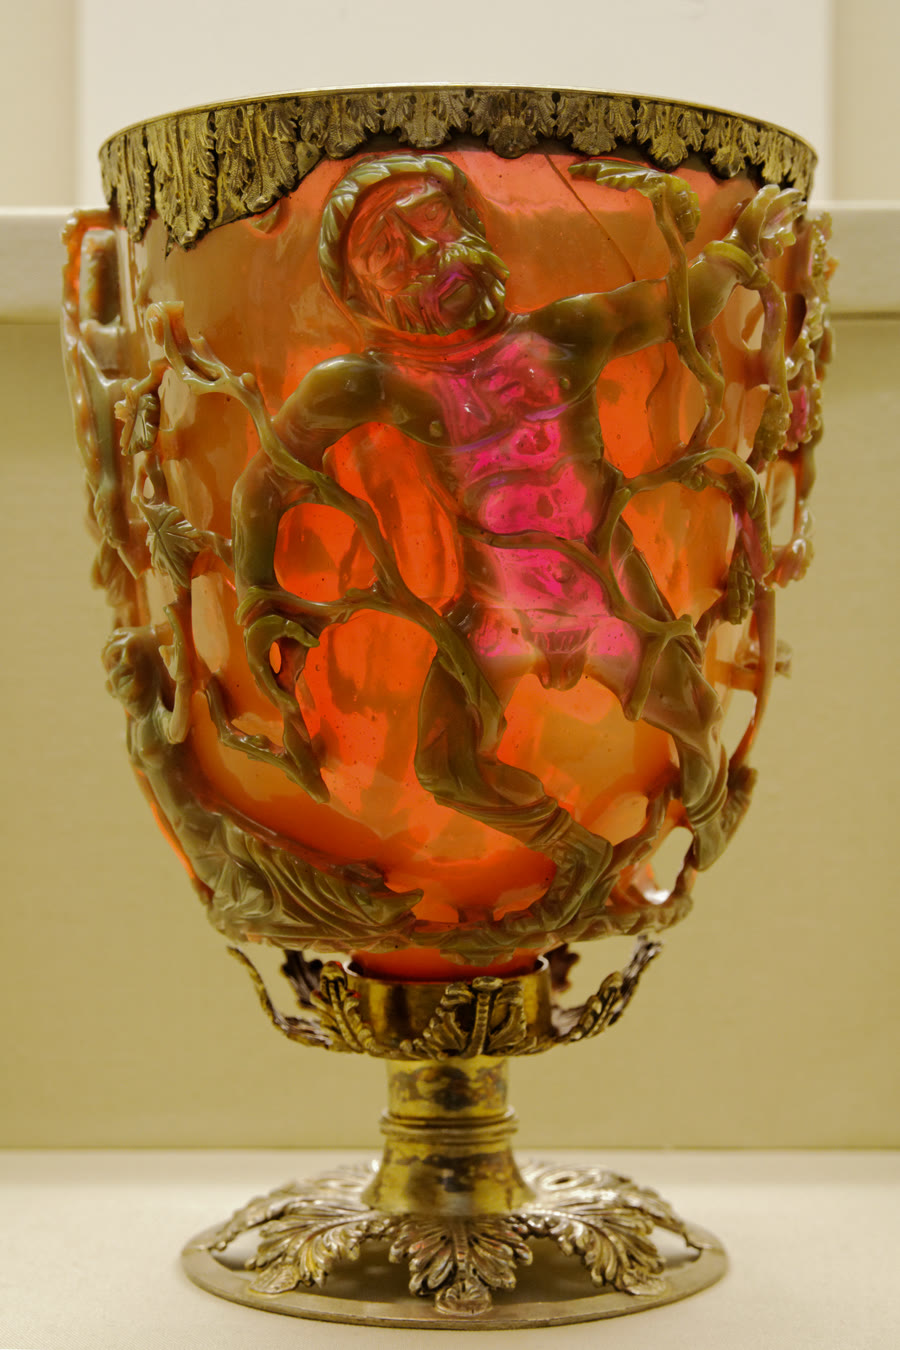
\includegraphics[width=0.32\linewidth]{images/book4/lycurgus-cup.jpg}

{\small La coupe de Lycurgue, un verre romain du \textsc{iv}\textsuperscript{e}~siècle,
éclairée de l'intérieur~: elle paraît verte en lumière réfléchie et rouge en
lumière transmise, effet de \omterm{def:b3:inorganic-materials:nano}{nanoparticules} d'or et d'argent dans le verre.
Photographie~: Marie-Lan Nguyen, CC BY 2.5.}
\end{omfigure}

\begin{history}[Des nanoparticules avant le mot, et un ballon de football en carbone]
Les verriers coloraient le verre en rouge avec de l'or bien avant que
quiconque sache pourquoi~; la coupe de Lycurgue en montre l'effet le plus
frappant. Michael Faraday prépara des \omterm{def:b3:colloids:colloid}{colloïdes} d'or dans les années 1850
et vit que leur couleur venait de particules trop petites pour être vues.
En 1985, Harold Kroto, Robert Curl et Richard Smalley, en vaporisant du
graphite au laser, découvrirent que les agrégats de soixante atomes de
carbone étaient exceptionnellement stables et proposèrent la cage fermée de
douze pentagones et vingt hexagones~; ils reçurent le prix Nobel de chimie
1996.
\end{history}

\section{Exercices}

\begin{exercise}[$\star$]\label{exo:b3:inorganic-materials:1}
Une couche de produit entre deux solides a une épaisseur de \qty{2.0}{\micro\metre} au bout de \qty{10}{h}. Au bout de
combien de temps atteindra-t-elle \qty{6.0}{\micro\metre}, si la croissance est parabolique~?
\end{exercise}

\begin{exercise}[$\star$]\label{exo:b3:inorganic-materials:2}
Écrire l'hydrolyse de l'orthosilicate de tétraéthyle en acide silicique, la
condensation de deux molécules d'acide silicique, et la réaction globale qui
donne la silice.
\end{exercise}

\begin{exercise}[$\star$]\label{exo:b3:inorganic-materials:3}
Classer $\ce{SiO2}$, $\ce{B2O3}$, $\ce{Na2O}$ et $\ce{CaO}$ en formateurs ou en \omterm{def:b3:inorganic-materials:glass}{modificateurs de réseau}, et dire ce que
$\ce{Na2O}$ fait au réseau de la silice.
\end{exercise}

\begin{exercise}[$\star$]\label{exo:b3:inorganic-materials:4}
Combien de pentagones et d'hexagones possède $\ce{C70}$~? Combien de liaisons~?
\end{exercise}

\begin{exercise}[$\star\star$]\label{exo:b3:inorganic-materials:5}
% ledger: rion:Sr2+XII, rion:Ca2+XII, rion:Ba2+XII, rion:Ti4+VI, rion:O2-VI
Calculer les \omterm{def:b3:inorganic-materials:perovskite}{facteurs de tolérance} de $\ce{SrTiO3}$, $\ce{BaTiO3}$ et $\ce{CaTiO3}$ avec les rayons en coordinence douze
de $\ce{Sr^2+}$ (\qty{144}{pm}), $\ce{Ba^2+}$ (\qty{161}{pm}) et $\ce{Ca^2+}$ (\qty{134}{pm}), $r(\ce{Ti^4+}) = \qty{60.5}{pm}$ et $r(\ce{O^2-}) = \qty{140}{pm}$. Que
prévoient-ils~?
\end{exercise}

\begin{exercise}[$\star\star$]\label{exo:b3:inorganic-materials:6}
Une \omterm{def:b3:inorganic-materials:zeolite}{zéolithe} X a pour formule anhydre $\mathrm{Na_{86}[(AlO_2)_{86}(SiO_2)_{106}]}$ (données de l'exercice).
Donner Si/Al et sa capacité d'échange pour $\ce{Ca^2+}$ en millimoles par gramme.
\end{exercise}

\begin{exercise}[$\star\star$]\label{exo:b3:inorganic-materials:7}
% ledger: lat:Au
L'or est cubique à faces centrées avec $a = \qty{407.8}{pm}$. Estimer le nombre de couches d'une
particule d'or cuboctaédrique d'environ \qty{5}{nm} de diamètre, son nombre
d'atomes et la fraction située en surface.
\end{exercise}

\begin{exercise}[$\star\star$]\label{exo:b3:inorganic-materials:8}
Un \omterm{def:b3:solid-state:classes}{semi-conducteur} a une \omterm{def:b3:solid-state:band}{bande interdite} massive de \qty{1.74}{eV}, et son électron et son \omterm{def:b3:solid-state:carriers}{trou} une \omterm{def:b3:quantum-model-systems:oscillator}{masse
réduite} de $0.10\,m_e$ (données de l'exercice). Estimer la couleur de la lumière émise par
des boîtes de rayon 2.0 et \qty{3.0}{nm}, en négligeant l'attraction coulombienne.
\end{exercise}

\begin{exercise}[$\star\star$]\label{exo:b3:inorganic-materials:9}
Les nanotubes $(10, 10)$, $(10, 0)$, $(9, 0)$ et $(12, 8)$ sont-ils métalliques ou \omterm{def:b3:solid-state:classes}{semi-conducteurs}~? Lesquels
sont de type fauteuil, lesquels de type zigzag~?
\end{exercise}

\begin{exercise}[$\star\star\star$]\label{exo:b3:inorganic-materials:10}
% ledger: cod:MOF5.formula, cod:MOF5.a, cod:MOF5.Z
Le MOF-5, $\mathrm{Zn_4O(C_8H_4O_4)_3}$, est cubique avec $a = \qty{25.82}{\angstrom}$ et huit unités formulaires par maille.
Calculer sa masse volumique. Si un gramme a une surface de $\qty{3000}{m^2}$ (données de
l'exercice), à combien de terrains de football de $\qty{105}{m} \times \qty{68}{m}$ cela correspond-il~?
\end{exercise}

\begin{exercise}[$\star\star\star$]\label{exo:b3:inorganic-materials:11}
À l'aide du décompte des couches de la \cref{prop:b3:inorganic-materials:magic},
montrer que la fraction en surface d'un agrégat cuboctaédrique tend vers $3/n$ pour $n$ grand, et
la comparer à la fraction exacte pour $n = 8$.
\end{exercise}

\begin{exercise}[$\star\star\star$]\label{exo:b3:inorganic-materials:12}
Une cage de carbone fermée, à trois liaisons par atome, contient $p$ pentagones, $h$ hexagones
et $s$ heptagones. Montrer que $p - s = 12$.
\end{exercise}

\section{Problème~: adoucir l'eau avec la zéolithe A}

\begin{problem}[{Problème du week-end --- adoucir l'eau avec la zéolithe A~: la
formule et la règle de Löwenstein, la capacité d'échange théorique, la
zéolithe nécessaire pour un lavage, et la fenêtre qui laisse entrer le
calcium et retient les détergents}]
\label{pb:b3:inorganic-materials:1}
% ledger: iza:LTA.formula, iza:LTA.window, aw:Na, aw:Al, aw:Si, aw:O, aw:H, aw:Ca, aw:C, rion:Ca2+VI
La \omterm{def:b3:inorganic-materials:zeolite}{zéolithe} A, utilisée dans les lessives à la place des phosphates, a pour formule
$\mathrm{Na_{12}[(AlO_2)_{12}(SiO_2)_{12}]\cdot 27H_2O}$ et des fenêtres de \qty{0.41}{nm} de diamètre. Une eau du robinet contient
\qty{2.0}{mmol/L} de $\ce{Ca^2+}$, et un lavage en utilise \qty{15}{L}~; pendant la durée d'un lavage, la \omterm{def:b3:inorganic-materials:zeolite}{zéolithe}
atteint 60\,\% de sa capacité (données du problème).

\medskip\noindent\textbf{Partie I --- La formule.}
\begin{enumerate}
  \item Calculer la masse molaire de la formule anhydre.
  \item Calculer celle de la formule hydratée.
  \item Donner Si/Al.
  \item Énoncer la règle de Löwenstein et ce qu'elle implique ici pour
        l'arrangement de Si et Al.
  \item Quelle est la charge de la charpente par formule~?
  \item Calculer la fraction massique d'eau dans la \omterm{def:b3:inorganic-materials:zeolite}{zéolithe} hydratée.
\end{enumerate}

\medskip\noindent\textbf{Partie II --- Capacité d'échange.}
\begin{enumerate}[resume]
  \item Écrire l'équilibre d'échange entre la \omterm{def:b3:inorganic-materials:zeolite}{zéolithe} sodique et les ions
        calcium.
  \item Combien d'ions $\ce{Ca^2+}$ une formule peut-elle fixer~?
  \item Calculer la capacité théorique de la \omterm{def:b3:inorganic-materials:zeolite}{zéolithe} anhydre en mmol de $\ce{Ca^2+}$
        par gramme.
  \item La calculer pour la \omterm{def:b3:inorganic-materials:zeolite}{zéolithe} hydratée.
  \item Exprimer la capacité anhydre en milligrammes de $\ce{CaCO3}$ par gramme, l'unité
        usuelle de la dureté de l'eau.
\end{enumerate}

\medskip\noindent\textbf{Partie III --- Un lavage.}
\begin{enumerate}[resume]
  \item Calculer la quantité de $\ce{Ca^2+}$ dans l'eau d'un lavage.
  \item Calculer la masse de \omterm{def:b3:inorganic-materials:zeolite}{zéolithe} hydratée nécessaire à la capacité
        théorique.
  \item La calculer à 60\,\% de la capacité.
  \item Calculer la masse de sodium libérée dans l'eau.
  \item Pourquoi les fabricants de lessives ont-ils remplacé les
        phosphates~?
  \item Pourquoi la \omterm{def:b3:inorganic-materials:zeolite}{zéolithe} A fixe-t-elle $\ce{Mg^2+}$ plus lentement que $\ce{Ca^2+}$~?
\end{enumerate}

\medskip\noindent\textbf{Partie IV --- La fenêtre.}
\begin{enumerate}[resume]
  \item Comparer la fenêtre au diamètre d'un ion $\ce{Ca^2+}$ (rayon en coordinence six
        \qty{100}{pm}).
  \item Que doit faire un ion $\ce{Ca^2+}$ hydraté pour passer~?
  \item Pourquoi un anion \omterm{def:b3:colloids:surfactant}{tensioactif} comme le dodécylsulfate reste-t-il à
        l'extérieur~?
  \item Que fait la \omterm{def:b3:inorganic-materials:zeolite}{zéolithe} A comme agent desséchant, et pourquoi
        l'appelle-t-on \omterm{def:b3:inorganic-materials:zeolite}{tamis moléculaire}~?
  \item Comment le remplacement de $\ce{Na+}$ par $\ce{K+}$ modifierait-il la taille des molécules admises~?
  \item Dans la ZSM-5, pourquoi le \textit{para}-xylène quitte-t-il les pores plus vite que l'\textit{ortho}-xylène~?
  \item Énoncer le résultat~: la capacité d'échange théorique de la
        \omterm{def:b3:inorganic-materials:zeolite}{zéolithe} A anhydre pour $\ce{Ca^2+}$.
\end{enumerate}
\end{problem}
